\chapter[Anomaly Detection for the Roman Space Telescope Wide Field Instrument's Science Data Processing Pipeline]{Anomaly Detection for the Roman Space Telescope Wide Field Instrument's Science Data Processing Pipeline}

\section{Abstract}
The Roman Space Telescope (RST) Wide Field Instrument (WFI) will be utilizing a preliminary Science Data Processing (SDP) pipeline during its Integration and Test, and to some extent during Operations, to track basic statistics and identify known features such as cosmic rays, snowballs as well as possible anomalies in raw detector data. 
In our detectors, these anomalies appear as jumps in the ramp of a readout and are classified as cosmic rays if they appear as a streak or snowballs if they're more circular. 
The WFI employs an array of 18 H4RG-10 detectors that collect image samples.
Each set of raw frames within a non-destructive exposure is packaged by the SDP pipeline into image cubes for each detector.
Each cube is a time series of $4096 \times 4096$ accumulating pixel frames.
The preliminary analysis pipeline is used to locate anomalies in these time-series accumulation frames and identify the type of anomaly, either natural phenomena or detector characteristic.
To compare different methods, we've implemented both heuristic-based and data-driven methods to identify anomalies.
For the heuristic-based approach, we identify snowballs and cosmic rays by the size and shape of outlier pixel clusters between consecutive frames.
For data driven methods, we evaluated a Convolutional Neural Network (CNN) model, and more traditional methods like Principal Component Analysis (PCA).
CNN is a supervised learning/classification method. 
Thus, we used a labeled dataset of anomalies to perform segmentation of the image and identify anomalies. 
We used previously identified cosmic rays and snowballs to measure the accuracy and efficiency of the mentioned approaches. 
In evaluating these methods, we aim to pick the best fit for the SDP pipeline's anomaly detection in terms of both performance and runtime. 

\section{Introduction}
The Roman Space Telescope (RST) Wide Field Instrument (WFI) employs an array of 18 H4RG-10 detectors to collect image samples.
Each detector on the WFI utilizes a up-the-ramp readout scheme that produces $4096 \times 4096$ pixel images at each frame along the exposure. 
For a given exposure, each frame gives us information on the amount of light collected over time and allows us to identify both the location and time of anomalies within a ramp.
During an exposure, natural or detector-related events may occur that affect groups (or sets) of pixels across the detector. 
Because we're collecting time-series information, we can see the exact frame that the event occurs and observe how the event affects subsequent frames. 
There are many different sources that might cause errors in our detectors' data, such as read noise patterns, thermal noise, compression errors, and software errors, but we are particularly interested in external and natural sources of errors \parencite{cillis2018snowballs}. 
Both cosmic rays and snowballs are transient events that result in sudden increases in charges and pixels’ Data Number (DN) values, compared to their typical neighboring pixels.
These events are also rare.
Therefore, we can use anomaly detection to identity these outliers.
Figure \ref{rst/fig:anomalies} shows examples of these two events.

\begin{figure}
    \centering
    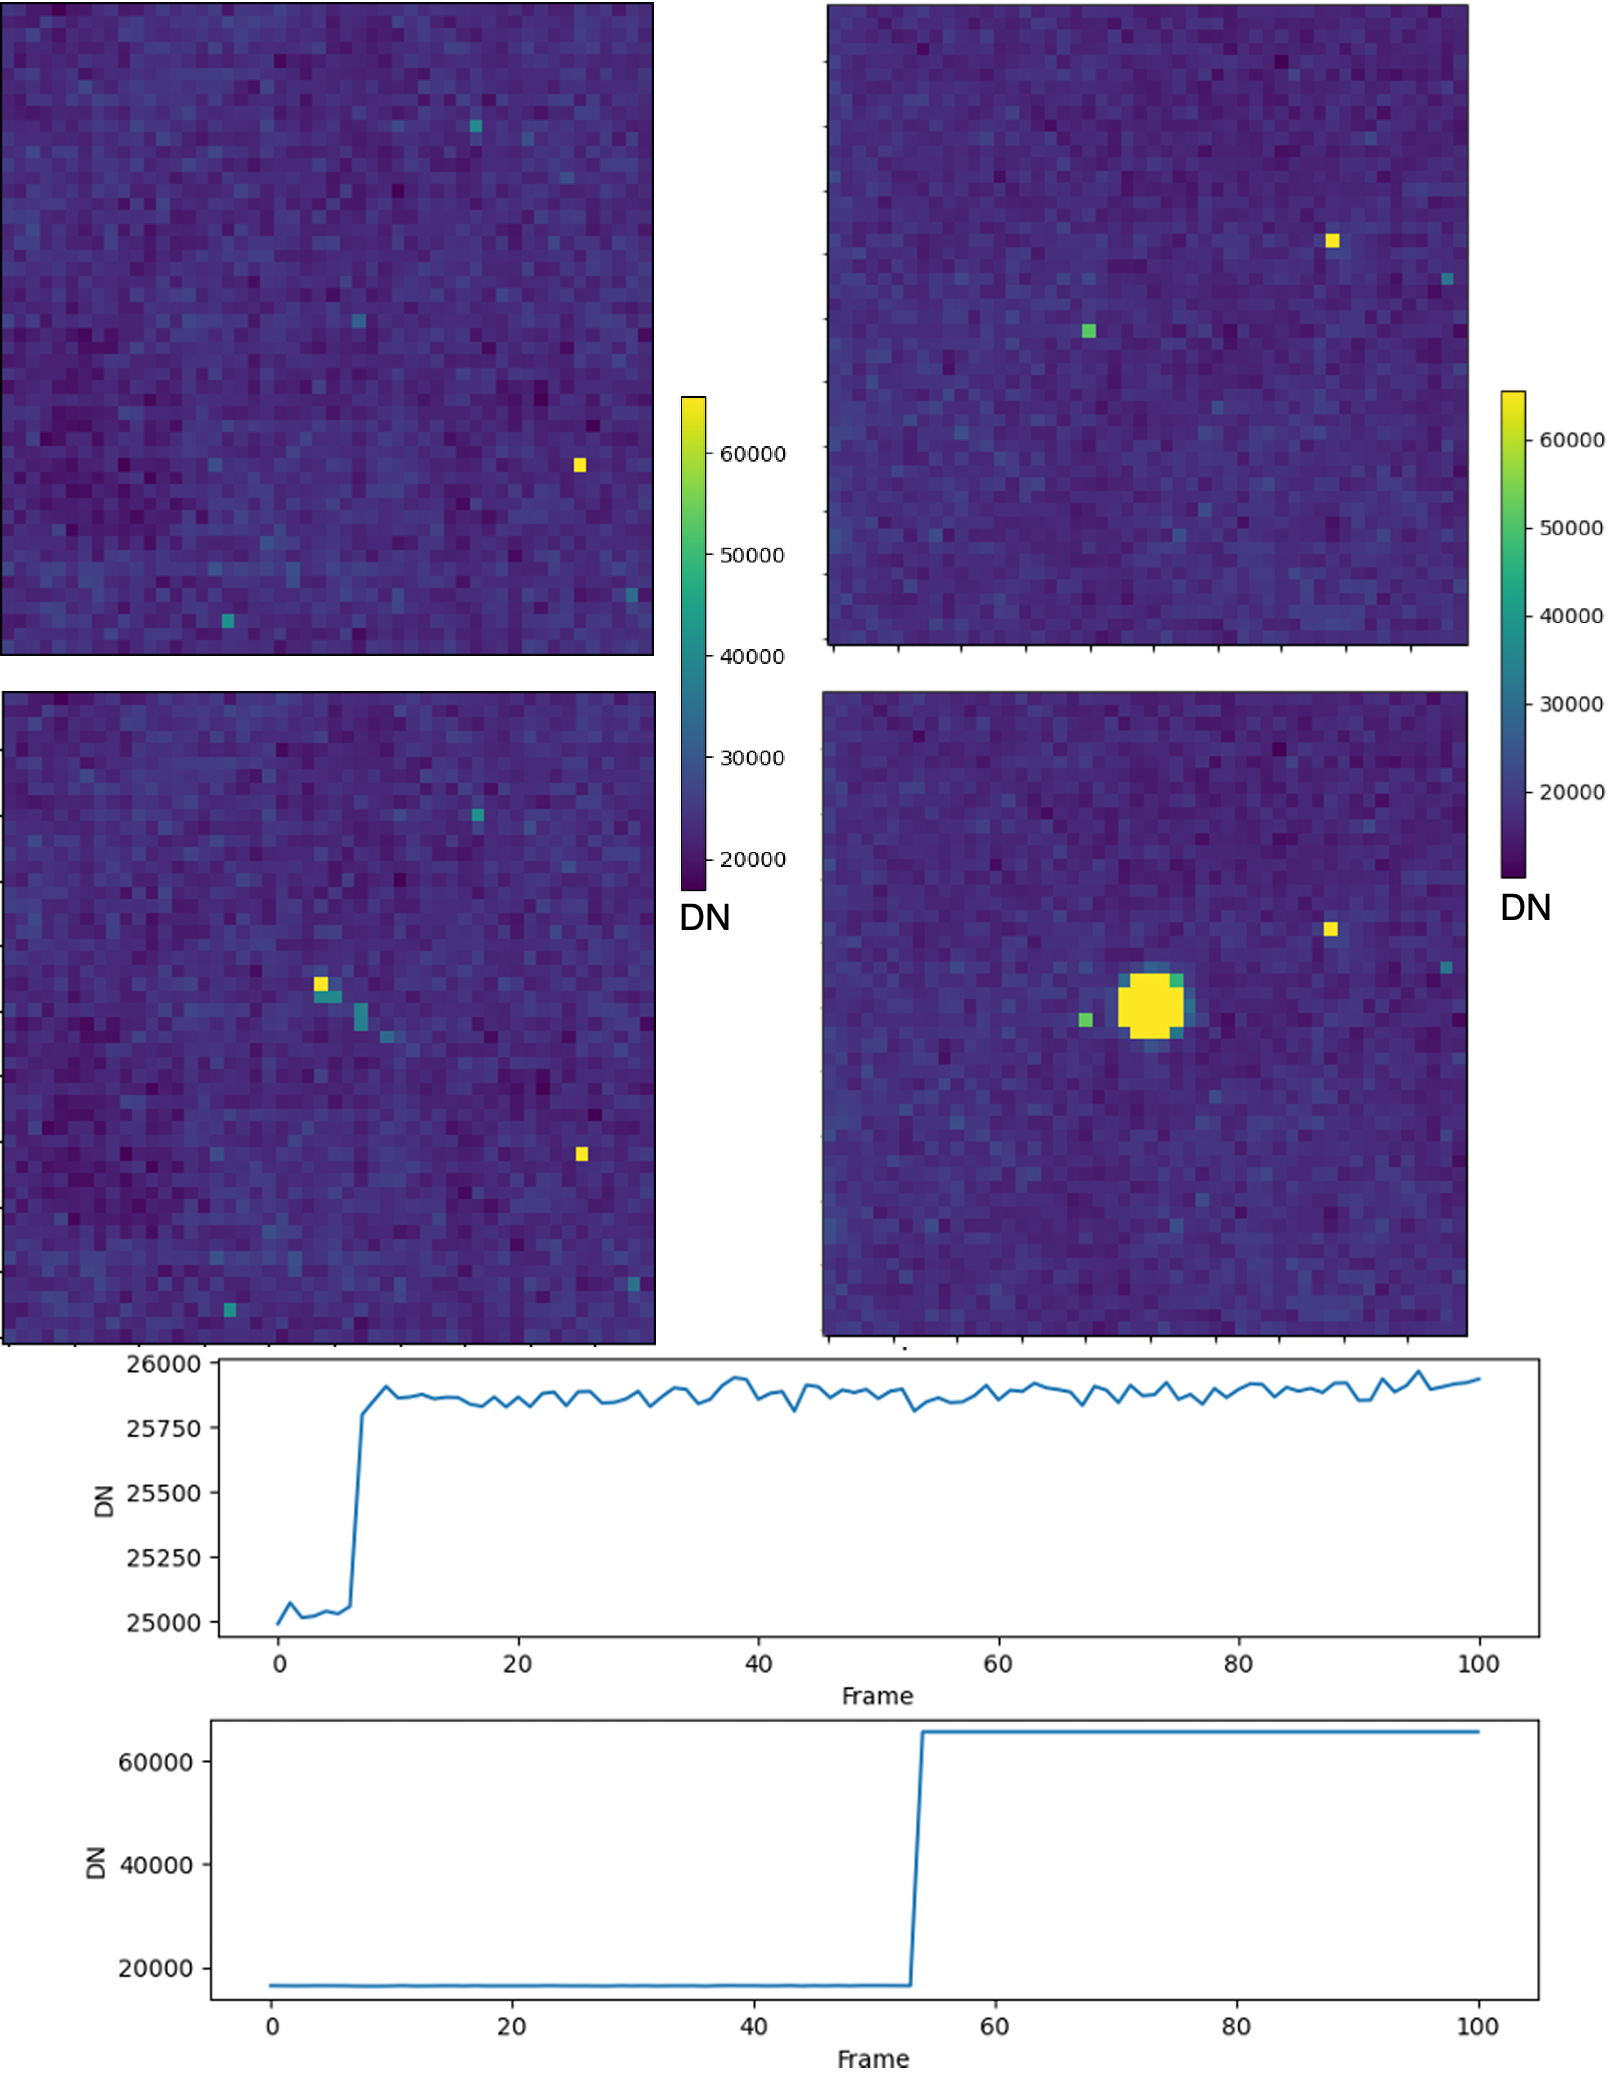
\includegraphics[width=.75\linewidth]{figs/rst/Examples_fixed.png}
    \caption{An example of a cosmic ray (left) and snowball (right) in RST's detector data. The top frames show the frame prior to the event and the bottom frames show the area after the event occurred. The bottom graphs show the overall DN value across the entirety of the exposure, showing large jumps at the time of the event for the cosmic ray (top) and snowball (bottom).}
    \label{rst/fig:anomalies}
\end{figure}

An anomaly is defined as an unexpected occurrence in a sequence based on a data set of typical sequences \parencite{horton2021integrating}. 
Given our image is mostly typical pixels, we can use this feature to identify out of distribution pixels that may be caused by snowballs or cosmic rays. 
While snowballs are a relatively newly recognized detector phenomenon, detection and rejection of snowballs are common practices for astronomical images \parencite{van2001cosmic}.
These cosmic rays appear as streaks across multiple pixels within an exposure as the incident cosmic ray imparts energy as a point spread function across neighboring pixels \parencite{pych2003fast}.

Both snowballs and cosmic rays will appear as jumps in DN value in a ramp but the shape of the affected neighboring pixels helps us differentiate between the two.
Snowballs will be circular in shape and affect 8 or more pixels \parencite{cillis2018snowballs}.
On the other hand, Cosmic Rays will be any grouping larger than 2 pixels that shows a linear streak. 

The goal of our anomaly detection is to highlight these features as part of the RST WFI SDP's pipeline. 
As such, SDP's processing time should keep up with data generation time so that we can identify issues within the detectors as we collect new data. 
This poses a challenge due to the massive data size of the data products from the array of 18 detectors. 
To address this challenge, raw data is automatically processed into interpretable products as part of the SDP pipeline. 
As this anomaly detection system will be part of the SDP pipeline as an additional data product, the runtime of any method must be taken into account along with the method's accuracy. 

The rest of this paper is organized as follows.
First we go over the methods for identifying and classifying snowballs and cosmic rays in Section \ref{rst/sec:methods}.
Then, in Section \ref{rst/sec:data} we explain the dataset chosen and how labels for the dataset were generated.
After that, we discuss the results of the different methods and draw conclusions about which methods to implement in the SDP pipeline in Section \ref{rst/sec:results}.
Finally, we go over future works in Section \ref{rst/sec:future}.

\section{Methods}
\label{rst/sec:methods}
To identify the anomalies in our data, we split our problem into two distinct tasks: 1) locating and grouping pixels that have irregular ramps and 2) classifying those pixels as cosmic rays, snowballs, or something else entirely.
By splitting our anomaly detection into two tasks, we can use the first step to identify regions of interest and reduce our search area for snowballs and cosmic rays to that of anomalous pixels.
This can drastically reduce the amount of pixels we have to classify as we also identify the frame that the anomaly occurred in, reducing our focus to a smaller window around the event. 
The following are potential candidate methods for accomplishing these two tasks.

\begin{table}
    \centering
    \begin{tabular}{|l|l|}
            \hline
        \textbf{Step 1: Locating Anomalies} & \textbf{Step 2: Classifying Anomalies} \\
                \hline

        & Heuristic Rules \\
        Statistical Thresholding& \parencite{cillis2018snowballs} \\
        \hline
        Principal Component Analysis (PCA) & Convolutional Neural Network (CNN)\\
        \parencite{cillis2018snowballs} & \parencite{gu2018recent} \\
                \hline

    \end{tabular}
    \caption{Methods for Locating and Classifying Anomalies}
    \label{rst/tab:methods}
\end{table}

There are other viable methods for accomplishing these tasks, such as Reed-Xiaoli (RX), Localized Reed-Xiaoli (LRX), and James Webb Space Telescope's (JWST) Bayesian Generalized Least Squares (GLS) for locating anomalies, but the scope of this work will focus on the methods in Table \ref{rst/tab:methods}.
RX is an unsupervised learning methods that uses a window around a test pixel to compare with the local background \parencite{reed1990adaptive}.
LRX is similar to RX but instead uses a double concentric window to compare the test pixel with a guarded local background \parencite{molero2013analysis}.
JWST's GLS estimator is also an unsupervised method that calculates the slope, or ramp, of each pixel along the time domain and determines the probability that discontinuities in the ramp occurred due to cosmic rays \parencite{robberto2015cr}.
Please note that the JWST data was constructed similarly to the RST's, resulting in non-destructive accumulating frames. 

Before any of the data is used for these methods, they must be loaded and pre-processed.
For more information about this and the dataset selection, see Section \ref{rst/sec:data}.

\subsection{Locating Anomalies}
\begin{figure}[b]
    \centering
    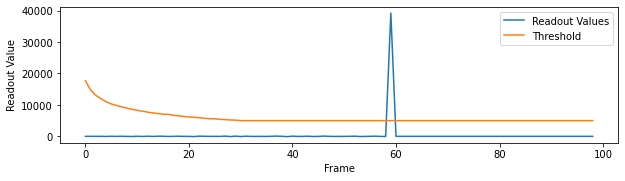
\includegraphics[width=1\linewidth]{figs/rst/Threshold.png}
    \caption{The readout values for a flagged pixel. The read out values are the amount of DN gained in a given frame. We compare this value to our calculated threshold and, if surpassed, that specific location and frame is flagged for classification.}
    \label{rst/fig:threshold}
\end{figure}
To locate the anomalies, we looked for methods that would be able to not only identify where a potential anomaly is located but when the event occurred that caused the anomaly. 
\subsubsection{Statistical Thresholding}
Our initial approach is readout thresholding, where we take two subsequent frames, $x_i$ and $x_{(i-1)}$ where $n$ is the number of frames in an exposure. 
For each readout frame $\Delta x_i$, we calculate the mean $\mu_i$ and standard deviation $\sigma_i$ across its pixels. 
We use these values to calculate the threshold for jumps in the ramp with a minimum threshold value of 5000 DNs.
\begin{equation}
    \Delta x_i > \max(\mu_i + 50 \sigma_i, 5000)
\end{equation}
These values were chosen for dark frames as they allow us to easily identify large jumps traditionally associated with snowballs or cosmic rays. 
From here, we create a pixel mask for each frame of all readout values that exceed this threshold. 
We then preform a series topological transformations to bridge and fill in incomplete holes through dilation, binary hole fill, and erosion procedures using SciPy's ndimage library \parencite{2020SciPy-NMeth}.
Finally, we remove any grouping of pixels of two pixels or less to ensure any jumps in the ramp we discover affect multiple pixels and then use scikit-image's measure library to locate the central pixel for each group \parencite{scikit-image}.
We are then left  with groupings of pixels that could potentially be either a cosmic ray or snowball.


\subsubsection{Principal Component Analysis (PCA)}
Given the majority of pixels within our image aren not affected by anomalies, we can use a random subset of pixels within an exposure and fit PCA to the ramps of these samples.
If we limit our principal components to two, we can create a fit for the majority of simple ramps. 
Using our PCA fit, we can reduce all of the pixels in our image to our latent space representation and then inverse transform them to compare the original and reconstructed result \parencite{wold1987principal}.
Examples of this are shown in Figure \ref{rst/fig:PCA}. 

\begin{figure}
    \centering
    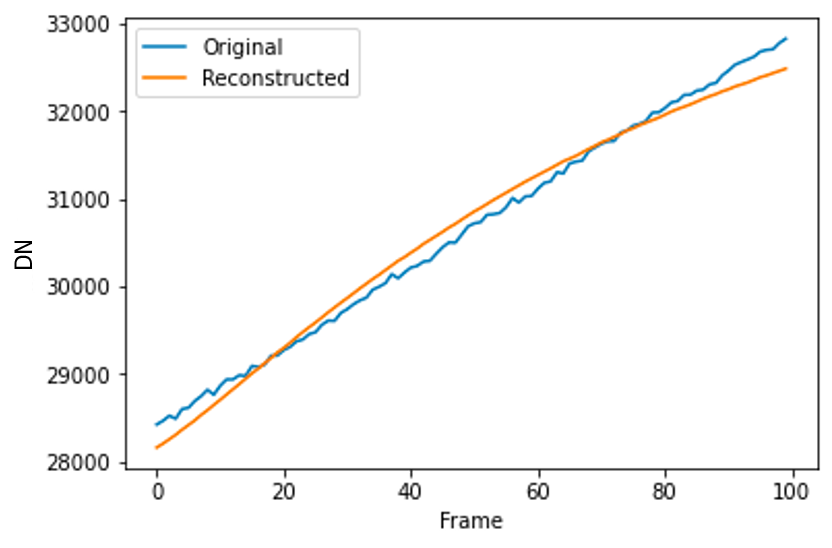
\includegraphics[width=0.49\linewidth]{figs/rst/PCA_Good.png}
    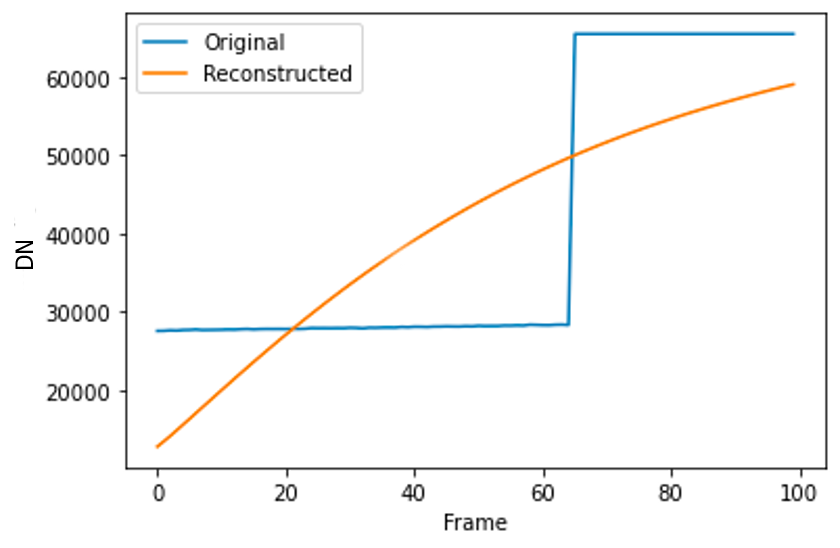
\includegraphics[width=0.49\linewidth]{figs/rst/PCA_Bad.png}
    \caption{Examples of reconstruction of ramps using PCA. The DN values for the reconstructed image are calculated by transforming the original values and then inverse transforming our original ramp using only a subset of the principal components (i.e. two) to reproduce the shape. By limiting the number of principal components to two, we can have the reconstructed image fit the shape fairly well for normal ramps and not fit ramps with anomalies.}
    \label{rst/fig:PCA}
\end{figure}

With the reconstructed values, we are able to calculate the residual ($Image_{Reconstructed} - Image_{Original}$) of the errors and identify where anomalies occur based on spikes in the ramp of the residual. 
To identify these spikes, we can employ a similar method to the Statistical Threshold method to calculate the change in residuals between each frame and find out of distribution values. 
This results in identifying the frames for each pixel that have large jumps in the residual. 
By limiting the number of PCA components to two, our reconstructed ramps will be relatively smooth, causing original ramps that have large jumps in them to have a large change in residual at the frame of the event.

Finally, like the statistical method, we create the pixel mask by highlighting any pixel whose change in residual is above the threshold.
We then identify regions using the same topological transformations and scikit-image's measure library for finding blobs \parencite{scikit-image}.

\subsection{Classifying Anomalies}
From the locating anomalies methods, we obtain a frame and pixel mask matrix containing information about potential anomalies with a ramp for each pixel in an exposure. 
We also obtain a table listing groupings of pixels to classify. We call this table the Event Table as it describes the time and location of potential anomalies. 
These groupings are the input into our classification methods as they help limit the search to specific pixels and frames across the exposure. 

\subsubsection{Heuristic Rules}
For heuristic rules, these groupings are labeled and measured by the number of pixels affected and the major and minor axes lengths of the affected area. 
We use these values to determine the type of anomaly.
Snowballs are large circular anomalies that cover 9 or more pixels.
Cosmic rays are oblong anomalies that cover more than 2 pixels. 
We determine the circularity of the anomaly be comparing the minor and major axis using the following criteria.
\begin{align*}
    \text{Circular:}\ &  \text{minor\_axis} \geq \text{major\_axis}/2 \\
    \text{Large:}\ & \text{area} \geq 9
\end{align*}

From this we are able to produce two output products: a new data cube where each frame is a mask identifying pixels affected by anomalies, and an updated Event Table with information about each anomaly. 

\subsubsection{Convolutional Neural Network}
\label{rst/sec:CNN}
For each listing in the Event Table, we take a 32 square pixel sample region around the central pixel spatially and the three frames around the event frame for a sample of $32 \times 32  \times 3$ pixels. 
This is the input into our CNN which is trained using hand labeled data from the DCL dataset. 
The CNN architecture processes input images through two convolutional layers followed by ReLU activations and max pooling, which flattens the output.
Finally we pass the output through two fully connected layers to produce class scores for None, Cosmic Rays, Snowballs, and Potential Anomalies classes based on the labeled dataset.
We preformed two tests with the CNN by training and testing on our all of the labeled dataset and just the data from the same detector to see how well the method generalizes. 
Both tests were preformed with an 80/20 test/train split with balanced classes. 
The output classes from the CNN are then used to label the pixels in the mask with their associated class and update the Event Table with anomaly labels. 
\subsection{Output Products}
To align with the rest of the products from the SDP pipeline, we package the outputs from the anomaly detection pipeline as Hierarchical Data Format 5 (HDF5) files \parencite{The_HDF_Group_Hierarchical_Data_Format}.
HDF5 is a file format that is designed to store large amounts of data and is perfect for the types of products we need to produce for the SDP.
Because of HDF5's efficient read/write procedures, the SDP is able to keep up with the data generation rate while producing analysis products. 
For each exposure, we produce three binary mask arrays for events labeled as Cosmic Rays, Snowballs, and Potential Anomalies for each pixel within a ramp. 
These binary masks are the same shape as the exposure and allow us to quickly identify and flag problem pixel/frame combinations in an exposure. 
We also produce a single image for each anomaly type where each pixel is the frame number of an event. 
This allows us to visualize anomalies and see how they may change throughout an exposure.
Finally, the Event Table is formatted so that each row in the HDF5 array is an anomaly that has central pixel, size, shape (semi-major and semi-minor axis), and classification as columns. 
These products are produced during SDP pipeline and added as part of the automated report. 
\section{Data}
\label{rst/sec:data}
The H4RG detectors used in the WFI array are able to perform non-destructive reads while producing an exposure resulting in measurements through time, also referred to as up-the-ramp measurements. 
This allows us to take the up-the-ramp measurements taken during an exposure and order them in a series to create frames within the exposure. 
This results in a time series of frames for each integration from a detector's pixel values being reset at the beginning of an exposure to the final accumulated pixel values at the end of an exposure \parencite{casertano2022determining}.
For testing the effectiveness of the anomaly detection pipeline, we will be utilizing real exposures taken during the selection phase of the flight detectors for the WFI detector array. 
During the selection phase of flight detectors, over 70 detectors went through numerous experiments with different types of light exposures, both bright and dark.
The dark tests consisted of a two-hour long exposure where detectors accumulated across 100 frames.
These tests are ideal to identify cosmic rays and snowballs due to their long exposure time, resulting in more opportunities for anomalies to appear in the frames. 
For the purposes of testing these methods, this paper focuses on using just these dark exposures. 

The data from these tests are provided in the form of Flexible Image Transport System (FITS) files that consist of 101 frames of $4096 \times 4096$ pixel images \parencite{wells1979fits}.
The first frame in an exposure is the reset frame and can be disregarded. 
The FITS data is loaded into a NumPy array of unsigned integers by iterating over the array \parencite{harris2020array}.
To correct the read direction of FITS data, the data is processed by subtracting every pixel values from the maximum possible DN value for each pixel, $2^{16} - 1$, across all frames.
This leaves us with a data cube of $100$ frames, each with $4096 \times 4096$ pixels. 

The data provided by the DCL lab contains labeled information about known snowballs during the exposure. 
These snowballs are our preliminary ground truth for identifying the effectiveness of our methods. 
In addition to these snowballs, the outputs for each method are reviewed to identify snowballs and cosmic rays that are not in the original labels
Because the heuristic method is overly sensitive, each anomaly highlighted by the method was hand labeled as potential anomaly, cosmic ray, snowball, or non-anomaly. 
These hand labels are used to measure the accuracy of each method and train methods such as the CNN in Section \ref{rst/sec:CNN}.

\section{Results and Conclusions}
\label{rst/sec:results}

As we are able to split our system into two different subsystems, the results here will discuss which of the methods are best for accomplishing each individual task. 
Then we will go more in depth with the best pairing of methods integration into the RST WFI SDP. 
For consistency, all of the tests were preformed on a 2021 M1 Macbook Pro Max with 64GB of unified memory.
Much of the development of this work was done on NASA Center for Climate Simulation PRISM GPU cluster. 

\subsection{Locating Anomalies}
The two methods we tested for locating anomalies were statistical thresholding and PCA.
Both methods look for large jumps in a time series but each method is looking for a different type of jump.
The statistical thresholding method is purely looking for jumps in the DN accumulated each frame by identifying large changes in DN compared to the rest of the accumulated DN in the frame. 
The PCA method trains on a subset of pixels across the exposure and is looking for large jumps in the residual error from transforming and inverse transforming each pixel. 
For performance, both methods require calculating the difference between values, a threshold, and then identifying groups of flagged pixels. 
On average, this takes about 2 minutes and 10 seconds for each dark image with 100 frames. 
Because the PCA methods needs to fit, transform, and inverse transform the entire exposure, running it adds on an average of 42 seconds to locating anomalies. 
This makes the Statistical Threshold method faster than PCA in every experiment due to PCA requiring pre-processing. 

\begin{figure}
    \centering
    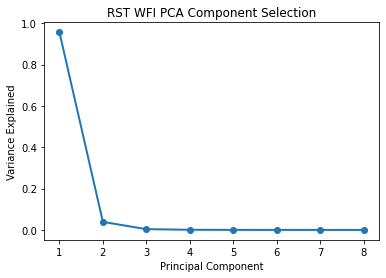
\includegraphics[width=.5\linewidth]{figs/rst/elbow.png}
    \caption{Elbow plot for the PCA method on typical ramps. A limit of 2 components was selected to ensure we aren't over fitting to the curve and missing anomalies.}
    \label{rst/fig:elbow}
\end{figure}

As for performance, both methods are over-sensitive to false positives.
The PCA method found less groupings than the statistical thresholding method but many of the omitted locations are false negatives.
We chose to use two principal components as any higher numbers of components would have fit to jumps in the ramp and caused lower errors.
Two components also gives us an overall shape that matches a typical ramp and explains most of the variance of the exposure's ramps without over fitting to the curve as shown in Figure \ref{rst/fig:elbow}.
This false negative rate varies from exposure to exposure but ranged from 65 to 80\% missed anomalies. 
Despite being overly sensitive to any jump in the ramp, the statistical thresholding method is preferred here due to it's higher accuracy and lower runtime.
This method had a false negative rate of 10\% across the entire labeled dataset of over 5000 hand labeled events. 
A method that filters most of the image without removing real anomalies is preferable to a method that filters more of the images including anomalies. The second step, Classifying Anomalies, can then label these false positives as None or Potential Anomaly. 
\subsection{Classifying Anomalies}
For classifying anomalies, we have the traditional method using heuristic rules around the shape of the grouping and a CNN trained on samples from the labeled anomalies. 
We utilized the output of the statistical thresholding method as the input into both of the classification methods. 
Neither method were spectacular at accomplishing the task but the heuristic rules method did outperform the CNN by a wide margin. 

We experimented with the CNN by training it on a subset of events in the Events Table that were hand labeled by humans and then testing it on a separate set of events. 
We tested training using a subset of all exposures in the labeled dataset as well as just exposures from a specific detector.
In both cases, we were unable to have the CNN generalize to different exposures. 
Because of the class imbalance and hard to differentiate nature of the dataset, the CNN would misclassify cosmic rays as potential anomalies and almost never correctly identify them as cosmic rays unless the streak was large enough to differentiate. 
The CNN was able to correctly classify snowballs about 50\% of the time, labeling them as potential anomalies in other cases. 
In the future, this method may be better suited than heuristic rules but further refining of the labeled dataset is necessary. 
As it stands, with the overlap between cosmic rays and potential anomalies, there is little room for improvement without further defining how we want to differentiate these classes. 

Heuristic rules outperformed our CNN method in both accuracy and runtime.
The outputs from Event Table in locating anomalies include measurements of the size and shape of the anomaly. 
This makes it very efficient to run through each entry of the table and pre-define a look up table to classify each anomaly. 
The time the heuristic rules pipeline takes to generate a report depends on the number of anomalies in the Event Table but, on average, it is able to classify 100 events from the Event Table a second. 

\subsection{SDP Pipeline Integration}
Of the methods tested, the best combination of methods for the SDP pipeline would be the Statistical Thresholding method for locating anomalies and the Heuristic Rules method for classifying anomalies.
This combination method was able to find every pre-labeled snowball from the original dataset and correctly identify 85 out of 137 (62\%) of hand labeled snowballs. 
The method also over classified cosmic rays by identifying many potential anomalies and non-anomalies as cosmic rays.
This is likely due to the less rigid criteria for identifying cosmic rays compared to snowballs.
Figure \ref{rst/fig:heuristic_confusion} shows the confusion matrix for the Heuristic Rules method with the located data from the Statistical Thresholding method.
This method is currently being used in the SDP pipeline to identify anomalies in the WFI detector data.

\begin{figure}
    \centering
    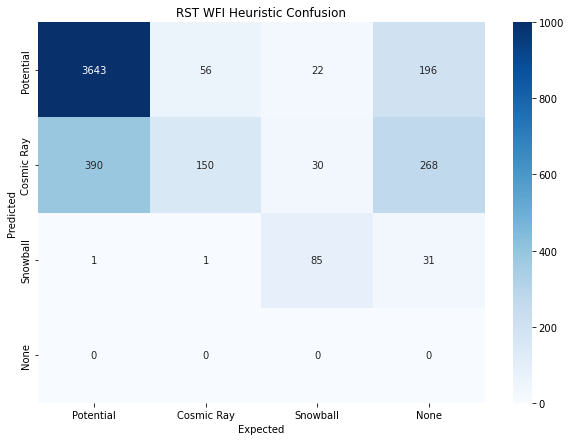
\includegraphics[width=.7\textwidth]{figs/rst/heuristic_confusion.png}
    \caption{Confusion matrix for the heuristic rules method with located data from statistical thresholding.}
    \label{rst/fig:heuristic_confusion}
\end{figure}

\section{Future Work}
\label{rst/sec:future}
This work is a preliminary analysis of the anomaly detection methods for the RST WFI SDP pipeline.
There are many areas for improvement and future work to be done.
First and foremost, more methods will need to be evaluated in order to determine a better alternative to the Heuristic Rules method for classification. 
The CNN method is a good candidate but needs more fine tuning to generalize to different exposures.
In addition to this, more labeled data will be needed to train the CNN and other methods, such as Mask RCNN or transformer-based architectures, particularly on illuminated data.
This labeled data could come from other tests if we were to generalize beyond just the dark exposures.
With a more well defined dataset of labeled data, we will be able to better assess the accuracy of these methods too. 

Another area for improvement may be finding better ways to locate anomalies.
We may revisit PCA to see if we can adjust the parameters (number of components and threshold for error) to reduce its false negative rate.
Additionally, other methods like RX, LRX and GLS, as described at the beginning of Section \ref{rst/sec:methods}, could be better suited for filtering the initial exposure.

The current implementation of the SDP pipeline uses a bad pixel mask to mask regions of the image that are problematic. 
Because we didn't have a bad pixel mask for the data we were using, we had to analyze the entire image with our anomaly detection methods.
This led to a large number of false positives from known bad pixels that appeared as anomalies in the dataset due to their sharp ramp in DN values at the beginning of the exposure.
In the future, we will need to integrate the bad pixel mask into the anomaly detection pipeline to filter out these false positives and use that to better assess the accuracy of the system. 

Finally, we will need to test the system on more than just dark exposures.
The current system is designed to work with dark exposures but we will need to adjust the system to work with other types of exposures that might have more difficult to detect anomalies.
There may not be a one size fits all solution to this problem but testing different types of exposures will help us determine the best methods for each type of exposure.